\documentclass[runningheads]{llncs}
\usepackage[utf8]{inputenc}
\usepackage[T1]{fontenc}
\usepackage{graphicx}

\usepackage{array}
\usepackage{booktabs}
\usepackage{tabularx}
\usepackage{longtable}
\usepackage{rotating}
\usepackage{pdflscape}
\usepackage[section]{placeins}
\usepackage{url}
\usepackage{xspace}
\usepackage{hyperref}
\usepackage{todonotes}
\usepackage[table]{xcolor}
\hypersetup{hidelinks}

\newcommand{\ie}{\textit{i}.\textit{e}.,\xspace}
\newcommand{\eg}{\textit{e}.\textit{g}.,\xspace}
\newcommand{\etal}{\textit{et al}.\xspace}
\newcommand{\vs}{\textit{v}.\textit{s}.\xspace}

% Selected works metadata (keep in sync with Section~\ref{sec:selected-works}).
\newcommand{\selectedWorkCount}{29}
\newcommand{\selectedWorkYearStart}{2003}
\newcommand{\selectedWorkYearEnd}{2025}
\newcommand{\selectedWorkYearRange}{\selectedWorkYearStart--\selectedWorkYearEnd}

% Table styling helpers (keep settings local by wrapping tables in {...}).
\newcommand{\kgTableSetup}{%
  \scriptsize%
  \setlength{\tabcolsep}{6pt}%
  \renewcommand{\arraystretch}{1.25}%
}
\newcommand{\kgLargeTableSetup}{%
  \scriptsize%
  \setlength{\tabcolsep}{3pt}%
  \renewcommand{\arraystretch}{1.15}%
}

\title{Knowledge Exploration in Knowledge Graphs: State of the Art, Taxonomy, and Open Challenges}
\titlerunning{KG Exploration in Knowledge Graphs}
\author{Task 2.4 group}
\authorrunning{Task 2.4}
\institute{Draft survey manuscript}

\begin{document}
\maketitle

\begin{abstract}
  The growing availability of Knowledge Graphs (KGs) has fueled research on interactive systems for exploring, querying, and making sense of graph-structured knowledge. This survey reviews the state of the art on \emph{knowledge exploration} in KGs, proposes a taxonomy of key design attributes (interaction paradigm, guidance strategy, visualization, backend assumptions, scalability, and evaluation), and analyses representative works spanning faceted browsing, relationship discovery, guided query building, and recommendation-based exploration. We also discuss practical tools with graphical user interfaces, commonly used datasets and evaluation protocols, provide selection guidance for practitioners, and outline open challenges and research directions.
\end{abstract}
\keywords{Knowledge graph exploration \and linked data visualization \and exploratory search \and user guidance \and faceted browsing \and relationship discovery \and SPARQL query building \and sense-making}

\noindent\fbox{%
  \parbox{\dimexpr\linewidth-2\fboxsep-2\fboxrule\relax}{%
    \textbf{Note regarding this draft:}
    \begin{itemize}
      \item The analyzed approaches (PDFs) are located in the \texttt{/paper} directory.
      \item Other related surveys are located in the \texttt{/survey} directory.
      \item The \texttt{website/} folder contains the React application code for the interactive survey companion.
    \end{itemize}
  }%
}
\vspace{1em}

\section{Introduction}
\label{sec:introduction}
Knowledge graph exploration aims to help users inspect, connect, and query linked data without requiring expertise in formal graph query languages (\eg SPARQL, Cypher). It can be seen as a form of exploratory search~\cite{marchionini2006,white2009} where information needs evolve during interaction (``berrypicking''~\cite{bates1989}). Graph representations support flexible navigation and rich semantics, but they also introduce major challenges: schema complexity, data heterogeneity, ambiguous labels, endpoint latency, and the need for \emph{guidance} that prevents users from getting lost in uninformative traversals or over-complex results. Beyond correctness, exploration systems must support an iterative \emph{sense-making} process where users progressively refine their information needs and interpretations.

\subsection{KG exploration: definitions, impact, and challenges}
In this survey, \emph{knowledge exploration} refers to interfaces and methods that enable users to:
\begin{itemize}
  \item find and filter entities/relations in a KG without writing formal queries from scratch;
  \item discover informative relationships and paths between entities (relationship discovery);
  \item receive suggestions for query expansions, next exploration steps, or suitable visualizations, ideally balancing relevance with diversity/novelty;
  \item obtain interpretable results through graphs, tables, maps, or natural-language (NL) feedback.
\end{itemize}
The core tension is balancing \emph{expressivity} and \emph{usability} while keeping interactive response times on large KGs (\eg DBpedia, Wikidata) and offering guidance that supports both \emph{accurate} retrieval and \emph{serendipitous}, diverse discovery.

\paragraph{Impact.} KG exploration lowers the entry barrier to graph-shaped knowledge by combining search, browsing, and guided query formulation.
\todo[inline]{TO COMPLETE}

\paragraph{Challenges.}
\todo[inline]{TO COMPLETE}

\subsection{Contributions and structure}
This manuscript contributes: (i) a practical taxonomy of KG exploration systems; (ii) a structured analysis of representative works; (iii) a comparative table highlighting key design choices; and (iv) a discussion of evaluation practices and open challenges. The remainder is organized as follows: scope and methodology (Section~\ref{sec:scope-methodology}), taxonomy (Section~\ref{sec:taxonomy}), sub-tasks (Section~\ref{sec:subtasks}), analysis of selected works (Section~\ref{sec:selected-works}), comparative discussion (Sections~\ref{sec:comparison}--\ref{sec:evaluation}), tools and benchmarks (Sections~\ref{sec:tools}--\ref{sec:gold-standards}), open issues (Section~\ref{sec:open-issues}), and conclusions (Section~\ref{sec:conclusions}).

\section{Scope and Methodology}
\label{sec:scope-methodology}
\subsection{Differences from related surveys}
Existing surveys cover Linked Data visualization and exploration systems, but differ in scope and in how they frame user guidance.
Dadzie and Rowe~\cite{2011_Dadzie_Approaches_to} propose a requirements-driven survey of Linked Data visualization aimed at intuitive data consumption and knowledge discovery. They compare 15 LD browsers (7 text-based and 8 visualization-based), with strong emphasis on the needs of different user types (technical vs.\ lay users) and on visualization/UI capabilities.

Marie and Gandon~\cite{2014_Marie_Survey_of} broaden the picture by reviewing 14 Linked Data exploration and discovery systems, spanning browsers, recommenders, and exploratory search systems. Their analysis is organized around system classes and ``desired effects'' (\eg overviews, explanations, and in-session memory/breadcrumbs), and it highlights opportunities for richer assistance and discovery-oriented features.

Jacksi et al.~\cite{2016_Jacksi_State_of} provide a feature- and technology-oriented review of more recent Linked Data exploration systems. From 28 collected candidates, they include 16 systems (8 Linked Data browsers and 8 exploratory search systems) and compare them along feature checklists (e.g., faceted navigation, query models, and result presentation).

In contrast, our survey focuses specifically on \emph{knowledge exploration} in KGs as an iterative sense-making process, with explicit attention to (i) \emph{interaction paradigms} (facets, navigation, relationship discovery, query building), (ii) \emph{guidance and recommendation} mechanisms (hard constraints, ranked suggestions, personalization, NL-based assistance), and (iii) how these choices relate to \emph{backend assumptions}, \emph{scalability techniques}, and \emph{evaluation} evidence. Table~\ref{tab:related-surveys} summarizes these differences.

\begin{landscape}
  \begin{table}[!htbp]
    \centering
    \caption{Comparison with closely related surveys on Linked Data visualization and exploration.}
    \label{tab:related-surveys}
    {\kgTableSetup
      \begin{tabularx}{\linewidth}{@{}
        >{\columncolor[gray]{0.95}\raggedright\arraybackslash\bfseries}p{2.7cm}
        >{\raggedright\arraybackslash}X
        >{\raggedright\arraybackslash}c
        >{\raggedright\arraybackslash}X
        >{\raggedright\arraybackslash}p{2.4cm}
        @{}}
        \toprule
        \rowcolor[gray]{0.9} \textbf{Survey}                                                                                                                                                                  & \textbf{Objective / scope} & \textbf{\# approaches} & \textbf{Comparison taxonomy} & \textbf{Guidance focus} \\
        \midrule
        This work                                                                                                                                                                                             &
        KG exploration (RDF and property graphs); taxonomy + open challenges; links interaction, backend assumptions, scalability, and evaluation; includes selection guidance and a corpus comparison table. &
        29 (10 anchors)                                                                                                                                                                                       &
        Yes: interaction paradigm, guidance, visualization, backend/data access, scalability, evaluation.                                                                                                     &
        Explicit (constraints, ranking, personalization, NL guidance).                                                                                                                                                                                                                                                       \\ \addlinespace
        Dadzie \& Rowe~\cite{2011_Dadzie_Approaches_to}                                                                                                                                                       &
        Linked Data visualization for intuitive consumption and knowledge discovery; emphasizes user types (technical vs.\ lay).                                                                              &
        15                                                                                                                                                                                                    &
        Requirements-driven; text-based vs.\ visualization-based LD browsers; UI/feature comparison.                                                                                                          &
        Mostly implicit; limited recommendation/guidance.                                                                                                                                                                                                                                                                    \\ \addlinespace
        Marie \& Gandon~\cite{2014_Marie_Survey_of}                                                                                                                                                           &
        Linked Data exploration and discovery systems (browsers, recommenders, exploratory search); highlights achievements and opportunities.                                                                &
        14                                                                                                                                                                                                    &
        Yes: system classes + ``desired effects'' (overviews, explanations, memory, assistance).                                                                                                              &
        Includes recommenders; query suggestions discussed but still limited.                                                                                                                                                                                                                                                \\ \addlinespace
        Jacksi et al.~\cite{2016_Jacksi_State_of}                                                                                                                                                             &
        Review of Linked Data exploration systems; feature and technology comparison of browsers and exploratory search systems.                                                                              &
        16 (from 28)                                                                                                                                                                                          &
        Feature/technology-oriented summary tables (LDB vs.\ ESS).                                                                                                                                            &
        Limited; guidance treated mainly as a feature (e.g., query suggestion).                                                                                                                                                                                                                                              \\
        \bottomrule
      \end{tabularx}
    }
  \end{table}
\end{landscape}

\subsection{Scope}
We focus on \emph{interactive} KG exploration systems, \ie user-facing methods and tools that support iterative sense-making over graph-structured data through navigation, guided query construction, recommendations, and visualization. We include both RDF graphs queried via SPARQL and property graphs queried via Cypher when the contribution primarily targets exploration. We exclude work whose primary focus is (i) KG construction and curation pipelines, (ii) ontology engineering and schema alignment, (iii) standalone question answering systems that return answers without an exploration workflow, and (iv) offline graph analytics without an interactive exploration interface.

\subsection{Methodology}
\paragraph{Identification.} We searched CrossRef and Semantic Scholar using keywords such as ``knowledge graph exploration'', ``graph query suggestion'', ``SPARQL query builder'', ``linked data browser'', and ``visualization recommendation''.
\paragraph{Screening.} We filtered results by peer-reviewed status, relevance to exploration (excluding pure ETL or isolated QA), and availability of a described method or interface.
\paragraph{Inclusion.} We retained works that (i) target exploration and not only exact query answering, and (ii) propose either a user-facing interaction model or a guidance/recommendation mechanism.
\paragraph{Selection.} We selected \selectedWorkCount{} representative works (\selectedWorkYearRange{}) as anchors for the taxonomy.

\todo[inline]{TO DO. COMPLETE THE SECTION.}
Section~\ref{sec:selected-works} and Table~\ref{tab:comparazione} also summarize additional tools and papers.
\paragraph{Limitations.} This survey is not intended as an exhaustive systematic review; instead, it uses a compact set of representative works as anchors, complemented by a broader ecosystem of tools and systems (Section~\ref{sec:tools}). Because datasets, tasks, and metrics vary widely across papers, some comparative statements necessarily follow the evidence reported in the literature rather than replicated experiments.

\section{Taxonomic analysis of KG exploration approaches}
\label{sec:taxonomy}
We characterize approaches along the following attributes; Table~\ref{tab:taxonomy} summarizes typical design choices, while Table~\ref{tab:comparazione} provides a comparative overview of representative systems and methods.
\begin{itemize}
  \item \textbf{Interaction paradigm}: faceted browsing; relationship/path discovery; click-based graph navigation; guided query building; query-by-example and query-expansion recommendation; visualization recommendation.
  \item \textbf{Guidance strategy}: none/implicit guidance; hard constraints (\eg only valid next steps); lexical/semantic suggestions; ranked recommendations; personalization; natural-language prompts and paraphrasing to reduce schema and language ambiguity.
  \item \textbf{Visualization}: node-link graphs; facet panels; tabular/list views; automatically suggested charts/maps; multi-perspective analytic views (\eg maps/timelines).
  \item \textbf{Backend and data access}: SPARQL endpoints and URI dereferencing (RDF), property-graph backends (Cypher), and the extent of precomputation/caching required for interactivity.
  \item \textbf{Scalability}: target KG size, candidate-generation strategies, and reported latency; many works rely on DBpedia, Freebase, or Wikidata-like KGs.
  \item \textbf{Evaluation}: controlled user studies (usability, time, insights); offline benchmarks for ranking/recommendation quality and efficiency; deployment evidence from portals and logs.
\end{itemize}

\begin{figure}[htbp]
  \centering
  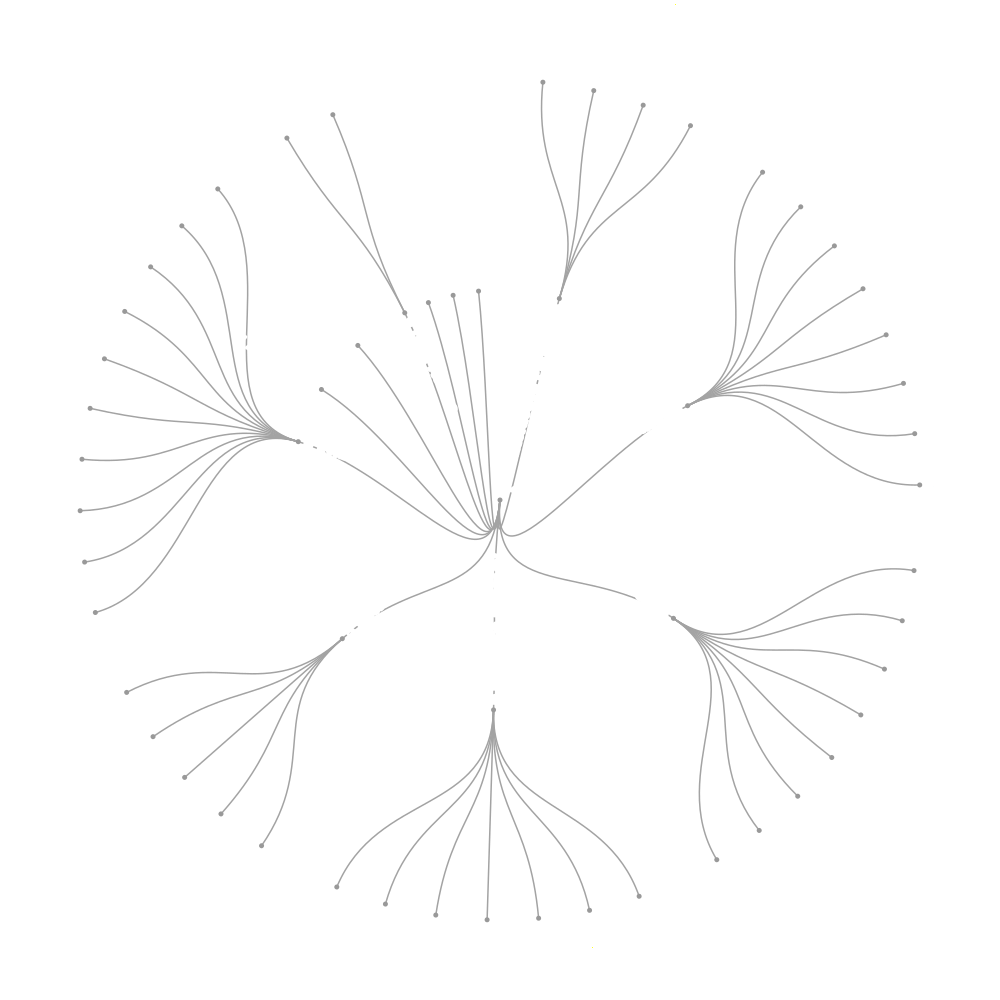
\includegraphics[width=\linewidth]{images/taxonomy}
  \caption{Visual representation of the taxonomy of interaction paradigms and guidance strategies.}
  \label{fig:taxonomy-visual}
\end{figure}

The resulting taxonomy dimensions are summarized in Table~\ref{tab:taxonomy}.
\begin{table}[!htbp]
  \centering
  \caption{Taxonomy dimensions for KG exploration interfaces and methods.}
  \label{tab:taxonomy}
  {\kgTableSetup
    \begin{tabularx}{\textwidth}{>{\columncolor[gray]{0.95}\bfseries}l X}
      \toprule
      \rowcolor[gray]{0.9} Dimension & Typical design choices                                                                                                                                   \\
      \midrule
      Interaction paradigm           & Faceted browsing; node-link navigation; relationship discovery; guided query construction; query-by-example and expansion; visualization recommendation. \\ \addlinespace
      Guidance strategy              & None/implicit; constraint-based suggestions (\eg valid-step); ranked recommendations; personalization; natural-language prompts and paraphrasing.        \\ \addlinespace
      Visualization                  & Node-link graphs; facets/panels; tables and lists; charts/maps; multi-perspective analytic views.                                                        \\ \addlinespace
      Backend and data access        & RDF/SPARQL endpoints and dereferencing; property graphs/Cypher; hybrid services; precomputation and caching for interactivity.                           \\ \addlinespace
      Scalability                    & From thousands to billions of triples/edges; strategies include sampling, summarization, efficient candidate generation, and incremental expansion.      \\ \addlinespace
      Evaluation                     & User studies (usability, time, insights); offline metrics for ranking/recommendation; deployment evidence from portals and logs.                         \\
      \bottomrule
    \end{tabularx}
  }
\end{table}

\section{Sub-tasks}
\label{sec:subtasks}
\subsection{Data preparation and profiling}
Several systems require profiling to extract facets (gFacet, Sampo-UI) or infer data types and roles to suggest appropriate views (LinkDaViz). Some tools rely on lightweight precomputation to keep response times interactive.

\subsection{Navigation and relationship discovery}
RelFinder~\cite{2009_Heim_RelFinder_Revealing} extracts relationship graphs between entities of interest; LodLive~\cite{2012_Camarda_LodLive_exploring} supports iterative node expansion across endpoints; Graph-Query Suggestions~\cite{2020_Lissandrini_Graph-Query_Suggestions} produces ranked expansion candidates for exemplar graph queries.

\subsection{Guided query formulation}
Sparklis~\cite{2017_Ferre_Sparklis_An} exposes only \emph{valid} refinement options given the current query state, and verbalizes the evolving query in controlled NL. Witschel et al.~\cite{2021_Witschel_Natural_Language-based,2022_Grether_Studying_Interaction} study and operationalize NL-based guidance for non-expert users.

\subsection{Recommendation and personalization}
LinkDaViz~\cite{2015_Thellmann_LinkDaViz_Automatic} recommends visualizations; the browser by Dur\~ao and Bridge~\cite{2018_Durao_A_Linked} uses a user profile (also expressed as Linked Data); Graph-Query Suggestions~\cite{2020_Lissandrini_Graph-Query_Suggestions} ranks candidate expansions using language-modeling and pseudo-relevance feedback over answer graphs.

\subsection{Visualization and analytics}
Sampo-UI~\cite{2022_Ikkala_Sampo-UI_A} combines faceted filtering with analytic perspectives (maps, timelines). LodLive and RelFinder emphasize node-link exploration, while gFacet and Sparklis combine structured panels and breadcrumb-like guidance to preserve readability.

\section{Analysis of selected works}
\label{sec:selected-works}
\subsection{Haystack}
Quan et al.~\cite{2003_Quan_Haystack_A} present Haystack, an early end-to-end platform for building end-user Semantic Web applications on top of arbitrary RDF data. The system combines (i) an RDF-centric programming environment (Adenine) for manipulating RDF content and services, and (ii) an extensible UI ontology (Ozone) for constructing \emph{views} that present RDF resources in familiar, application-like forms (e.g., for documents, email, tasks). By representing not only data but also UI specifications and logic in RDF, Haystack aims at network-updatable, extensible, and customizable applications in the spirit of the Semantic Web.

\emph{Takeaway.} Haystack anticipates many later KG exploration concerns (presentation, authoring, extensibility) by treating RDF as a unifying substrate for both data and interaction, at the cost of a substantial platform investment.

\subsection{Tabulator}
Berners-Lee et al.~\cite{2006_Berners-Lee_Tabulator_Exploring} introduce Tabulator, a generic browser for the Web of linked RDF data that follows dereferenceable URIs and supports serendipitous cross-domain reuse. The system provides an outliner (tree-like) view for incremental inspection of heterogeneous graphs, plus alternative views (tables, map, calendar/timeline) when results contain spatial/temporal properties. Tabulator also supports query-by-example: users can select cells/fields in the outliner to form graph patterns that are translated into queries (and can be inspected/edited as SPARQL). The paper emphasizes provenance awareness and extensible views, and frames the work as an exploratory platform rather than a completed usability-evaluated product.

\emph{Takeaway.} Tabulator establishes core interaction patterns for Linked Data browsing (follow-your-nose, multi-view inspection, query-by-example), but also highlights the UI and performance challenges of open-ended exploration across the Web of data.

\subsection{/facet}
Hildebrand et al.~\cite{2006_Hildebrand_facet_A} propose /facet, a faceted browser designed for \emph{heterogeneous} Semantic Web repositories. The key challenges addressed are (i) supporting different facet sets for different resource types, including selecting resources of one type using facets from semantically related types; (ii) automatically configuring facets from an arbitrary RDFS dataset without manual setup; and (iii) complementing hierarchical browsing with search to handle large hierarchies not designed for navigation. The system is positioned both as an ``instant interface'' for developers and as a starting point that can be refined into an end-user tool.

\emph{Takeaway.} /facet shows how faceted exploration can be made adaptive and (partly) self-configuring for multi-type RDF datasets, while exposing the difficulty of robust facet mining and hierarchy handling in the wild.

\subsection{gFacet}
gFacet~\cite{2008_Heim_gFacet_A} targets browsing of RDF data on the Web by combining node-link visualization with faceted filtering. The prototype is implemented in Flash and queries data via SPARQL; facets are shown as nodes connected by labeled edges, laid out with a force-directed algorithm, and can be pinned to stabilize the layout during interaction. Its core idea is to represent \emph{facets} and their (possibly hierarchical) values as first-class graph elements, so that selecting a facet value propagates filtering constraints through the graph while keeping the user in control of the visible result set. This design bridges two common exploration styles: free graph traversal and controlled multi-dimensional filtering.

The paper reports a small user study (10 participants) with three increasingly demanding tasks on music-related data, aimed at assessing whether users understand and purposefully apply \emph{graph-based facets}. Eye tracking and questionnaires suggest that prior familiarity with faceted browsing has a strong impact on success rates, pointing to a learnability gap and the need for onboarding and clearer affordances.

\emph{Takeaway.} gFacet demonstrates that faceted interaction can tame graph complexity, but it also shows that mixing graph navigation with facet logic requires careful design to remain self-explanatory to non-experts.

\subsection{Explorator}
Ara\'ujo et al.~\cite{2009_Araujo_Experimenting_with} study Explorator, a direct-manipulation RDF browser and querying tool grounded in a \emph{set-based navigation} model. Users manipulate sets of RDF resources/triples through operations such as projection and intersection, combining browsing, search, and query building to answer concrete questions while learning the domain. The paper reports a pilot study (six users with basic RDF knowledge) and a small qualitative experiment (four users) on two datasets (mobile phones and geopolitical data), highlighting recurring difficulties with schema discovery (classes vs.\ instances, finding properties) and UI affordances, but also showing that participants could construct nontrivial queries once the set metaphor was understood.

\emph{Takeaway.} Explorator demonstrates that set-based direct manipulation can support exploratory querying over RDF, but effective guidance for schema/vocabulary discovery and careful UI signaling are essential to avoid conceptual and interaction breakdowns.

\subsection{RelFinder}
RelFinder~\cite{2009_Heim_RelFinder_Revealing} addresses the task of discovering relationships between two entities in large RDF knowledge bases exposed through SPARQL endpoints (\eg DBpedia). Instead of relying on trial-and-error graph traversal, RelFinder automatically extracts a relationship graph by issuing an iterative sequence of SPARQL queries with increasing path length. To keep paths feasible and understandable, the algorithm constrains patterns such that the direction of property relations changes at most once; it also provides pragmatic parameters such as cycle suppression, regular-expression filtering of properties/entities, optional omission of structural predicates (\eg \texttt{rdf:type}), maximum path length, and endpoint configuration.

The tool is implemented in Adobe Flex/Flash and includes a defensive disambiguation step for mapping user terms to KG entities. The UI incrementally displays relationships starting from the shortest ones and includes interactive features (highlighting, previewing, filtering) to reduce clutter and support systematic inspection. This division of labor---automatic search plus interactive pruning---aligns well with exploratory relationship analysis, but the constrained path patterns and endpoint dependency illustrate the classic trade-off between completeness and interactivity.

\emph{Takeaway.} RelFinder exemplifies algorithmic assistance for relationship exploration: it shifts the bottleneck from manual traversal to controllable search and visualization, at the cost of restricting the search space for usability and performance.

\subsection{LodLive}
LodLive~\cite{2012_Camarda_LodLive_exploring} focuses on making Linked Data resources accessible through a lightweight, user-friendly node-link interface driven by SPARQL endpoints. A key engineering choice is that it runs as a JavaScript client without an application server, issuing JSONP calls to configured endpoints. Users start from a resource and progressively expand the neighborhood by following outgoing and incoming properties (including inverse links), building a session-level exploration context. A distinctive goal is interoperability: the tool is designed to navigate across multiple endpoints by leveraging \texttt{owl:sameAs} links; it also collects images and geospatial information for gallery/map views, and can parse dereferenced RDF resources via Sesame to create a temporary, single-resource endpoint.

Compared to systems that provide ranked suggestions, LodLive offers limited algorithmic guidance: it primarily supports \emph{direct manipulation} exploration (expand, inspect, repeat) and relies on visual representation and interaction workflow (history/session state) rather than explicit ranking or recommendation. This makes it a useful baseline for pure graph navigation, but dense nodes and heterogeneous schemas can quickly overwhelm non-expert users.

\emph{Takeaway.} LodLive represents the ``pure navigation'' paradigm: strong accessibility and interoperability, but little explicit guidance when users face large branching factors or unclear next steps.

\subsection{Payola}
Kl\'imek et al.~\cite{2013_Klimek_Payola_collaborative} present Payola, a collaborative framework for Linked Data analysis and visualization aimed at end users without SPARQL expertise. Payola separates a web-based client (analysis editing and result visualization) from a Scala-based server (user management, endpoint querying, data manipulation) and relies on a plugin ecosystem: analyses are built by connecting \emph{analyzer} plugins (roughly corresponding to SPARQL query building blocks), and results are rendered by \emph{visualizer} plugins that can be shared and reused. The paper illustrates the approach with use cases (including public procurement) and emphasizes extensibility and reuse as the primary contribution.

\emph{Takeaway.} Payola frames KG exploration as a configurable pipeline of reusable analyzers and visualizations; its effectiveness hinges on the availability of high-quality plugins and on keeping generated queries efficient.

\subsection{YASGUI}
Rietveld and Hoekstra~\cite{2013_Rietveld_YASGUI_Not} introduce YASGUI, a web-based SPARQL client intended to lower the friction of interacting with RDF endpoints. The system integrates practical features familiar from modern developer tooling: syntax highlighting/checking, autocompletion, endpoint lookup, query persistence, permalinks, and results rendering/download, with explicit attention to robustness when external services are unavailable.

\emph{Takeaway.} While not an ``exploration UI'' in the narrow sense, YASGUI is a foundational building block for KG exploration workflows by making iterative querying and debugging more accessible and reproducible.

\subsection{LD Viewer}
Lukovnikov et al.~\cite{2014_Lukovnikov_LD_Viewer} present LD Viewer, a customizable presentation framework for Linked Data resources that generalizes the earlier DBpedia Viewer. A central mechanism is the Triple Action Framework (TAF), which supports dataset-specific customization and interactive actions on presented triples (beyond static property-value rendering). The paper reports tests on DBpedia and LinkedGeoData and a preliminary user survey (10 responses) indicating generally positive impressions but also usability gaps (e.g., overlooked filtering features).

\emph{Takeaway.} LD Viewer shows how configurable ``resource pages'' can become interactive exploration surfaces; however, making advanced controls discoverable and robust across datasets remains challenging.

\subsection{LODmilla}
Micsik et al.~\cite{2014_AMA_LODmilla_Shared} propose LODmilla, a JavaScript/HTML5 Linked Data browser focusing on ``commodity'' features for generic LOD exploration: graph-based navigation across multiple datasets, graph manipulation, searching, and (distinctively) saving and sharing explored graph views. The goal is to preserve provenance and context for resources and enable collaborative sharing of exploration results.

\emph{Takeaway.} LODmilla extends graph navigation with reusable, shareable exploration artifacts, which supports collaboration but also raises the usual scalability and visual-clutter challenges of node-link interfaces.

\subsection{rdf:SynopsViz}
Bikakis et al.~\cite{2014_Bikakis_rdfSynopsViz_a} present rdf:SynopsViz, a framework for hierarchical visual exploration and analysis of Linked Data. The core idea is to construct multi-level hierarchies that group resources based on property values (automatically from data distributions or user-defined), enabling abstraction/summarization and efficient on-the-fly statistics via aggregation over hierarchy levels. The framework integrates faceted filtering, multiple visualization types (e.g., charts, timeline, treemap), and dataset metadata/quality indicators.

\emph{Takeaway.} Hierarchical summarization coupled with statistics can mitigate information overload in Linked Data visualization, but depends on robust grouping strategies and meaningful defaults for heterogeneous datasets.

\subsection{Sgvizler}
Skj{\ae}veland~\cite{2015_Skjaeveland_Sgvizler_a} introduces Sgvizler, a lightweight JavaScript wrapper that embeds SPARQL \texttt{SELECT} queries directly into HTML pages and renders their result sets into visualizations (charts, maps, timelines, graphs) using a common table abstraction (Google DataTable). Sgvizler emphasizes ease of integration, a large catalog of visualization types (notably via Google Chart Tools), and extensibility through custom renderers.

\emph{Takeaway.} Sgvizler provides a pragmatic bridge from SPARQL result sets to web visualizations, but it does not solve higher-level exploration problems such as selecting informative slices, mappings, or views.

\subsection{VIIQ}
Jayaram et al.~\cite{2015_Jayaram_VIIQ_auto-suggestion} present VIIQ, a visual interface for interactive graph query formulation over heterogeneous graphs. The system aims to reduce the vocabulary burden by recommending ranked edge (and label) suggestions for partially constructed query graphs, operating both passively (automatic top-$k$ suggestions) and actively (user-triggered ranked choices). The paper is presented as a demo focusing on UI features and the edge suggestion mechanism.

\emph{Takeaway.} VIIQ exemplifies suggestion-augmented visual query construction: ranked recommendations can make exact query graphs more approachable, but recommendation quality and explainability become central UX requirements.

\subsection{LinkDaViz}
LinkDaViz~\cite{2015_Thellmann_LinkDaViz_Automatic} tackles a recurring obstacle in KG exploration: choosing \emph{how} to visualize a slice of Linked Data and \emph{how} to bind data fields to visualization parameters. The proposed workflow guides users from selecting data to exploring it through recommended visualizations. Technically, LinkDaViz performs heuristic profiling of the selected data (scale/role inference), maps it into an internal input data model, and uses an explicit visualization model to generate candidate bindings (\eg which property should map to x-axis, series, geographic coordinates). These bindings are scored and ranked, producing a list of suggested chart configurations that users can refine. The paper describes a JavaScript-based web application with an Ember.js front-end and a Node.js back-end (using D3/Dimple and Leaflet visual components), accepting RDF and CSV data.

The evaluation combines usability and effectiveness. A user study with 20 participants covers seven tasks (selection, parameter assignment, exploration, customization, saving, and re-slicing data) and includes measures of perceived difficulty, UI impression, satisfaction, and the ``meaningfulness'' and coverage of generated visualizations. The paper also reports scalability tests across datasets and deployment environments.

\emph{Takeaway.} LinkDaViz demonstrates that visualization recommendation can lower the entry barrier for exploration, but also highlights the need for explainable recommendations and robust profiling in the presence of noisy schemas and heterogeneous data types.

\subsection{Sapphire}
El-Roby et al.~\cite{2016_El-Roby_Sapphire_Querying} present Sapphire, a system that helps users construct expressive SPARQL queries over public endpoints without requiring detailed prior knowledge of dataset vocabularies and literal encodings. Sapphire positions itself between ambiguous keyword search and expert-only SPARQL by (i) suggesting query terms based on the queried data and (ii) recommending query changes using a predictive user model, supporting an iterative refinement workflow.

\emph{Takeaway.} Sapphire illustrates a mixed-initiative path toward making SPARQL usable at scale; its practical success depends on reliable data-driven suggestions and user trust in automatic query repairs.

\subsection{A Linked Data Browser with Recommendations (LDRec)}
Dur\~ao and Bridge~\cite{2018_Durao_A_Linked} augment Linked Data browsing with personalized recommendations. The underlying premise is that both the data and the user profile can be represented as Linked Data, and that recommendations can be framed as a neighborhood-based prediction problem: given a user and a browsing context, which nearby resources should be suggested next?

Their main contribution is \emph{LDRec}, inspired by the Iterative Classification Algorithm. Candidate resources are classified using a local one-class classifier (based on nearest neighbors among positively labeled ``liked'' items); predicted labels are temporarily inserted into the graph as RDF triples and the classification is iterated, enabling preference signals to propagate through the neighborhood. The paper evaluates the method using both offline experiments (using a Linked Open Data-enabled recommender benchmark based on Facebook ``likes'' reconciled to DBpedia) and a user trial with 100 participants, reporting improved hit rates over a simpler non-iterative baseline and significantly higher user satisfaction.

\emph{Takeaway.} LDRec is a representative learning-based approach to personalization for exploration, but it raises practical issues such as cold-start profiles, privacy of preference data, and the cost of repeated neighborhood extraction on live endpoints.

\subsection{Sparklis}
Sparklis~\cite{2017_Ferre_Sparklis_An} aims to reconcile the expressivity of SPARQL with the usability of faceted exploration. The system maintains a state composed of the current query and a focus position; at each step, it computes context-specific suggestions (entities, classes, properties, operators) from the current query and its results, and applies query transformations selected by the user. A distinctive design choice is \emph{valid-step guidance}: Sparklis only proposes refinements that are guaranteed to return non-empty results, effectively preventing syntax and vocabulary/schema errors from surfacing to the user.

Sparklis verbalizes both the evolving query and the resulting answers in controlled natural language (English/French) and supports a large subset of SPARQL~1.1 features (\eg optional, negation, filters, aggregation, ordering). It requires no endpoint-specific configuration by discovering schema information on the fly, and it has been deployed as a portable web application (\url{http://www.irisa.fr/LIS/ferre/sparklis/}). Evaluation evidence includes controlled experiments and user studies (as reported in the Sparklis line of work) and analysis of anonymous usage logs over hundreds of users and more than a hundred endpoints.

\emph{Takeaway.} Sparklis demonstrates how strong, schema-aware guidance can make complex querying feasible for non-experts; however, always maintaining non-empty results may bias exploration away from hypothesis testing via intentionally empty queries.

\subsection{PICASSO}
Huang et al.~\cite{2017_Huang_PICASSO_exploratory} demonstrate PICASSO, an exploratory search system for connected subgraph substructure queries over graph databases consisting of multiple small/medium-sized graphs. The system supports progressive visual formulation of query graphs, incremental evaluation of successive refinements, and a multi-stream ``results wall'' that juxtaposes query-revision steps and their outputs to help users spot patterns and decide next exploration directions.

\emph{Takeaway.} PICASSO emphasizes that exploratory graph search benefits from explicit support for query evolution and result comparison across iterations, not only from faster subgraph matching.

\subsection{ViziQuer}
Cerans et al.~\cite{2018_Cerans_ViziQuer_A} present ViziQuer, a web-based diagrammatic query tool that provides visual counterparts for most SPARQL~1.1 \texttt{SELECT} constructs, including aggregation and subqueries. Queries are expressed in a UML-style notation over a configured schema/endpoint; the tool supports both instance-level and statistics queries and provides demo query environments. A preliminary experiment with 14 undergraduate students (SQL background, no SPARQL training) reports higher task completion for the visual group than for a textual SPARQL group.

\emph{Takeaway.} ViziQuer suggests that sufficiently expressive visual notations can reduce the barrier to writing complex SPARQL queries, especially for users comfortable with diagrammatic/SQL-like representations.

\subsection{LOD Explorer}
Jacksi et al.~\cite{2018_Jacksi_LOD_Explorer} present LOD Explorer, a client-side web application for exploring SPARQL endpoints through a combined node-link view and a details panel. The tool emphasizes ease of use for non-specialists: starting from resource search (with autocomplete), users can open multiple resources as nodes, inspect literals and incoming/outgoing connections, and follow links to expand the graph; the implementation uses JavaScript (JSONP calls), jQuery, and a graph drawing toolkit.

\emph{Takeaway.} LOD Explorer offers a lightweight, practical baseline for endpoint-centric graph navigation, but provides limited guidance beyond expand-and-inspect interaction.

\subsection{RDF Explorer}
Vargas et al.~\cite{2019_Vargas_RDF_Explorer} demonstrate RDF Explorer, a visual query builder that lets users incrementally construct SPARQL graph patterns while exploring the underlying data. Users start from keyword search, drag resources into a visual query canvas, and add edges/variables guided by existing properties between nodes; the tool exposes the evolving SPARQL query and aims to avoid interactions that lead to empty results while still supporting expressive patterns (including cycles).

\emph{Takeaway.} RDF Explorer exemplifies ``explore while you build'': tight coupling between navigation and query authoring can make expressive querying feasible for non-experts if suggestion generation remains responsive.

\subsection{Graph-Query Suggestions}
Lissandrini et al.~\cite{2020_Lissandrini_Graph-Query_Suggestions} focus on exploratory search via \emph{exemplar} graph queries, where users provide an example entity or edge and seek similar structures. The paper formalizes \emph{graph query suggestion} as ranking candidate expansion edges that complement a partial query. To support this, the authors adapt classical information-retrieval language modeling and pseudo-relevance feedback to knowledge graphs by representing queries and answers as bags of edge labels (augmented with neighborhood label information) and ranking expansions using KL-divergence-based scores.

The approach is evaluated on very large Freebase snapshots (76M nodes and 314M edges) using queries derived from QALD-7 and compared against popularity- and proximity-based baselines (\eg Personalized PageRank). Ranking quality is assessed with human relevance judgments collected via crowdsourcing (four-point scale; $>$25k judgments, at least three per query-suggestion pair). Results show that naive frequency/popularity heuristics often yield uninformative suggestions, while KL-divergence with pseudo-relevance feedback produces relevant expansions even from minimal initial queries and remains efficient at scale.

\emph{Takeaway.} This work provides a principled, unsupervised ranking model for interactive exploration without labeled logs; the remaining challenge is presenting and explaining expansions so users can select them confidently.

\subsection{S-Paths}
Destandau et al.~\cite{2021_Destandau_S-Paths_Set-based} introduce S-Paths, a browsing tool that shifts exploration from single resources to \emph{sets} of resources described through \emph{semantic paths} (multi-hop predicate chains). Starting from a set, the system identifies candidate paths and automatically selects readable views by aggregating end values and choosing suitable visual encodings, enabling comparison and context without repeated follow-your-nose navigation. The paper reports qualitative evaluation with different personas (publishers, reusers, lay users), emphasizing learning and novelty in dataset discovery.

\emph{Takeaway.} S-Paths complements resource-centric browsing with set-based, path-driven, aggregated views that help users understand ``what is typical'' and ``what is unusual'' in a dataset.

\subsection{Fast Approximate Autocompletion (FAAS)}
de la Parra and Hogan~\cite{2021_Parra_Fast_Approximate} study the efficiency--relevance trade-off in autocompletion for SPARQL query builders. They propose FAAS, an approach that builds a graph summary to \emph{over-approximate} suggestions that are likely to produce non-empty results, enabling tractable, responsive autocompletion on very large KGs. Experiments on a Wikidata dump show that FAAS can avoid endpoint timeouts and return suggestions within a few seconds, at the cost of reduced precision (median precision reported around 0.21).

\emph{Takeaway.} Approximate, locally indexed autocompletion is a viable way to keep interactive query building usable at Wikidata scale, but requires careful ranking and UX design to mitigate noisy suggestions.

\subsection{Natural language-based user guidance}
Witschel et al.~\cite{2021_Witschel_Natural_Language-based} study a sequential question-answering paradigm for KG exploration. Users first obtain entry points via keyword search; then, at each step, they select a set of nodes as context and ask a natural-language question, which is parsed and translated into a Cypher query. The system returns the answer as a new subgraph, enabling iterative refinement and exploration. To mitigate schema unawareness and natural-language ambiguity, the system provides recommended questions once a context is selected.

In a qualitative user study on a medical KG (10 medical-informatics students), the recommendation-enhanced version reduces time spent struggling with tool functionalities and increases the number of distinct insights discovered (average 5.4 vs.\ 3.4). At the same time, recommendations can introduce new failure modes (\eg users prematurely firing queries without selecting an adequate multi-node context), emphasizing that recommendation quality and context management are central to the UX.

\emph{Takeaway.} NL-based guidance can improve recall and reduce friction, but it must be tightly integrated with context selection and quality-controlled recommendations to avoid confusion.

\subsection{Studying interaction patterns}
Grether and Witschel~\cite{2022_Grether_Studying_Interaction} complement system-level contributions with a deeper analysis of user interaction patterns and intents. The paper reports two qualitative data collection phases on a medical exploration scenario (basic anamnesis) using a prototype tool and KG, involving eight final-year medical students. The first phase observes breakdowns with guidance disabled and then introduces support features (query recommendations and result previews); the second phase tests a subset of guidance hypotheses by iterating on the prototype.

The study emphasizes intent recognition from interaction traces and proposes concrete guidance mechanisms grounded in observed breakdowns (\eg better support for context selection, targeted recommendations, and feedback that exposes missed opportunities).

\emph{Takeaway.} Improving KG exploration requires aligning guidance mechanisms with real user intents and failure patterns; purely algorithmic enhancements are insufficient without understanding interaction behavior.

\subsection{Sampo-UI}
Ikkala et al.~\cite{2022_Ikkala_Sampo-UI_A} present Sampo-UI, a full-stack JavaScript framework for semantic portals based on the ``Sampo'' model: shared ontology infrastructure, multiple perspectives on the same KG, and a two-step user cycle (filter then analyze). Architecturally, Sampo-UI couples a React+Redux client with a Node.js/Express backend that generates SPARQL queries based on configuration, integrates multiple endpoints and external APIs, and maps SPARQL JSON results into developer-friendly objects; the API is documented and validated with OpenAPI. The framework is published on GitHub under the MIT license.

A case study on the WarVictimSampo 1914--1922 portal reports two faceted perspectives (war victims and battles), rich result-set visualizations (tables, maps, charts, temporal animations), and deployment evidence (opened in November 2019, nearly 20{,}000 unique users in the first month). The contribution is primarily engineering and reuse: it packages patterns for faceted selection, perspective switching, and analysis views into reusable components that can be adapted to new domains.

\emph{Takeaway.} Sampo-UI illustrates how to industrialize KG exploration as reusable portal components; effectiveness depends on domain modeling quality, indexing/search configuration, and long-term maintenance of the KG infrastructure.

\subsection{A User-Friendly SPARQL Query Editor}
Emonet et al.~\cite{2025_Emonet_A_User-Friendly} propose an easy-to-deploy SPARQL query editor powered by lightweight endpoint metadata. Built as an extension of YASGUI, the editor automatically renders query examples, provides context-aware autocomplete (including within \texttt{SERVICE} clauses) based on observed triple patterns, and offers a data-aware schema visualization; deployment is simplified via a custom HTML element.

\emph{Takeaway.} Metadata-driven query editors can reduce per-endpoint configuration effort and improve guidance quality for SPARQL-savvy users, but depend on the availability and freshness of endpoint metadata.

\section{Comparison table}
\label{sec:comparison}
Table~\ref{tab:comparazione} provides a comparative overview of KG exploration tools, methods, and supporting components in our local corpus (\texttt{paper/}).
\begin{landscape}
  {\kgLargeTableSetup
    \setlength{\LTleft}{0pt}
    \setlength{\LTright}{0pt}
    \begin{longtable}{@{}
      >{\columncolor[gray]{0.95}\raggedright\arraybackslash\bfseries}p{0.115\linewidth}
      >{\raggedright\arraybackslash}p{0.09\linewidth}
      >{\raggedright\arraybackslash}p{0.13\linewidth}
      >{\raggedright\arraybackslash}p{0.13\linewidth}
      >{\raggedright\arraybackslash}p{0.115\linewidth}
      >{\raggedright\arraybackslash}p{0.15\linewidth}
      >{\raggedright\arraybackslash}p{0.08\linewidth}
      >{\raggedright\arraybackslash}p{0.08\linewidth}
      @{}}
      \caption{Comparison of KG exploration tools, methods, and supporting components in the local corpus (\texttt{paper/}).}
      \label{tab:comparazione}                                                                                                                                                                                                                                                                                                                                                                       \\
      \toprule
      \rowcolor[gray]{0.9}
      \textbf{Work}                                                                  & \textbf{Primary goal}                            & \textbf{User interaction}                       & \textbf{Guidance}                                     & \textbf{Output}                     & \textbf{Backend \& assumptions}                             & \textbf{Evidence}    & \textbf{Availability} \\
      \midrule
      \endfirsthead
      \caption[]{Comparison of KG exploration tools, methods, and supporting components in the local corpus (continued).}                                                                                                                                                                                                                                                                            \\
      \toprule
      \rowcolor[gray]{0.9}
      \textbf{Work}                                                                  & \textbf{Primary goal}                            & \textbf{User interaction}                       & \textbf{Guidance}                                     & \textbf{Output}                     & \textbf{Backend \& assumptions}                             & \textbf{Evidence}    & \textbf{Availability} \\
      \midrule
      \endhead
      \midrule
      \multicolumn{8}{r}{\emph{Continued on next page}}                                                                                                                                                                                                                                                                                                                                              \\
      \endfoot
      \bottomrule
      \endlastfoot
      Haystack~(2003)~\cite{2003_Quan_Haystack_A}                                    & Platform (end-user Semantic Web apps)            & Configurable views; RDF authoring               & View/interaction model encoded in RDF (Ozone)         & Application-like views              & Local RDF store; extensible services (Adenine)              & System               & Paper/prototype       \\
      Tabulator~(2006)~\cite{2006_Berners-Lee_Tabulator_Exploring}                   & Generic Linked Data browser                      & Follow URIs; outliner; query-by-example         & Multi-view inspection; QBE$\rightarrow$SPARQL         & Outliner; tables; map; timeline     & URI dereferencing + SPARQL; open web                        & System               & Prototype/tool        \\
      /facet~(2006)~\cite{2006_Hildebrand_facet_A}                                   & Faceted browsing for heterogeneous RDF           & Facets per type; cross-type facets; search      & Auto facet configuration; prune empty refinements     & Facets + lists                      & RDF store + (S)PARQL; facet mining                          & Prototype            & Online demo           \\
      gFacet~(2008)~\cite{2008_Heim_gFacet_A}                                        & Faceted graph browsing                           & Graph + facets; pin/layout                      & Facet filtering                                       & Graph + facets                      & RDF/SPARQL; Flash client                                    & User study           & Demo (Flash)          \\
      Explorator~(2009)~\cite{2009_Araujo_Experimenting_with}                        & Direct manipulation RDF browsing/querying        & Set operations + browsing/search                & Set-based model (limited explicit guidance)           & Set panels; tabular results         & RDF store; set/projection operators                         & User studies         & Demo (web)            \\
      RelFinder~(2009)~\cite{2009_Heim_RelFinder_Revealing}                          & Relationship discovery                           & Select 2 entities; inspect paths; filters       & Constrained path search + interactive pruning         & Relationship graph                  & SPARQL endpoints; Flash/Flex                                & Case/demo            & Demo (Flash)          \\
      LodLive~(2012)~\cite{2012_Camarda_LodLive_exploring}                           & Lightweight Linked Data navigation               & Expand nodes; follow in/out links; sameAs jumps & None/implicit                                         & Graph; map/gallery                  & Client JS + JSONP; SPARQL endpoints                         & Demo/adoption        & Open source (MIT)     \\
      Payola~(2013)~\cite{2013_Klimek_Payola_collaborative}                          & LD analysis + visualization framework            & Compose analyzer pipelines; reuse plugins       & Plugin ecosystem (analyzers/visualizers)              & Pipelines + visualizations          & Scala server + SPARQL endpoints                             & Use cases            & Online tool           \\
      YASGUI~(2013)~\cite{2013_Rietveld_YASGUI_Not}                                  & SPARQL client for iterative querying             & Textual SPARQL editing                          & Autocomplete; endpoint lookup; syntax aids            & Editor + result rendering           & SPARQL endpoints; web services                              & Feature comparison   & Web tool              \\
      LODmilla~(2014)~\cite{2014_AMA_LODmilla_Shared}                                & Generic LOD graph browsing + sharing             & Graph navigation; save/share views              & None/implicit                                         & Graph + shareable views             & SPARQL endpoints; multi-dataset browsing                    & Prototype            & Paper/prototype       \\
      rdf:SynopsViz~(2014)~\cite{2014_Bikakis_rdfSynopsViz_a}                        & Hierarchical exploration + analytics             & Facets; hierarchy drill-down                    & Auto hierarchy + on-the-fly stats                     & Charts/timeline/treemap + stats     & RDF input (+ optional OWL); hierarchy construction          & Prototype            & Online prototype      \\
      LD Viewer~(2014)~\cite{2014_Lukovnikov_LD_Viewer}                              & Linked Data presentation framework               & Resource pages; filters; triple actions         & Triple Action Framework (configurable actions)        & Rich entity pages; map; filters     & SPARQL + optional index; dataset-specific actions           & User survey          & Paper/framework       \\
      Sgvizler~(2015)~\cite{2015_Skjaeveland_Sgvizler_a}                             & Visualize SPARQL result sets in web pages        & Embed \texttt{SELECT} in HTML                   & None/implicit                                         & Charts/maps/timeline/graphs         & SPARQL endpoints; DataTable abstraction                     & System/tool          & Open source (MIT)     \\
      VIIQ~(2015)~\cite{2015_Jayaram_VIIQ_auto-suggestion}                           & Visual graph query formulation                   & Draw query graph interactively                  & Ranked edge/label suggestions                         & Query graph builder UI              & Heterogeneous graph; query graphs                           & Demo                 & Paper/demo            \\
      LinkDaViz~(2015)~\cite{2015_Thellmann_LinkDaViz_Automatic}                     & Visualization recommendation                     & Select data slice; refine bindings              & Profiling + ranked binding suggestions                & Charts + maps                       & RDF/SPARQL (and CSV); visualization model                   & User study + perf.   & Online tool           \\
      Sapphire~(2016)~\cite{2016_El-Roby_Sapphire_Querying}                          & Assisted SPARQL query writing                    & Iterative query construction                    & Data-driven suggestions; query change recommendations & SPARQL queries + answers            & Public SPARQL endpoints                                     & System/demo          & Paper                 \\
      Sparklis~(2017)~\cite{2017_Ferre_Sparklis_An}                                  & Guided SPARQL query builder                      & Stepwise refinements; focus-based editing       & Valid-step (non-empty) + controlled NL                & Tables + NL verbalization           & SPARQL endpoints; on-the-fly schema discovery               & Studies + logs       & Online tool           \\
      PICASSO~(2017)~\cite{2017_Huang_PICASSO_exploratory}                           & Exploratory subgraph search                      & Progressive visual query; multi-stream wall     & Query evolution + result juxtaposition                & Results wall; subgraph views        & Graph DB over many small/medium graphs                      & Demo                 & Paper/demo            \\
      ViziQuer~(2018)~\cite{2018_Cerans_ViziQuer_A}                                  & Diagrammatic SPARQL authoring                    & UML-style visual queries                        & Schema-aware environment; visual constructs           & SPARQL incl.\ aggregates/subqueries & SPARQL endpoint + schema exploration service                & Experiment           & Open source           \\
      LDRec~(2018)~\cite{2018_Durao_A_Linked}                                        & Personalized Linked Data browsing                & Browse + user profile (likes)                   & Profile-based recommendations (ICA-inspired)          & InfoBox + recommended resources     & Linked profiles + SPARQL (DBpedia); neighborhood extraction & Offline + user trial & Paper                 \\
      LOD Explorer~(2018)~\cite{2018_Jacksi_LOD_Explorer}                            & Simple endpoint-centric exploration              & Search/autocomplete; open nodes; expand links   & Autocomplete + search within opened resources         & Graph + details panel               & Client JS + JSONP; SPARQL endpoints                         & Tool paper           & Online demo           \\
      RDF Explorer~(2019)~\cite{2019_Vargas_RDF_Explorer}                            & Visual SPARQL query builder                      & Drag resources; draw edges/variables            & Data-driven property suggestions; avoid empty results & Visual query + SPARQL view          & SPARQL endpoints (e.g., Wikidata)                           & Demo                 & Online + code         \\
      Graph-Query Suggestions~(2020)~\cite{2020_Lissandrini_Graph-Query_Suggestions} & Ranked query expansion for exemplar queries      & Start from exemplar; select expansions          & LM/PRF-ranked edge expansions                         & Suggested expansion edges           & Freebase snapshot (very large); IR scoring                  & Offline + crowd      & OA (CC-BY)            \\
      S-Paths~(2021)~\cite{2021_Destandau_S-Paths_Set-based}                         & Set-based exploration via semantic paths         & Select set; choose path/view                    & Automatic view selection + aggregation                & Aggregated set views                & SPARQL endpoint; path analysis                              & User study           & Demo + code           \\
      FAAS~(2021)~\cite{2021_Parra_Fast_Approximate}                                 & Fast approximate autocomplete for query builders & Autocomplete variables during query build       & Graph summary (over-approx. suggestions)              & Autocomplete lists                  & Local index over Wikidata dump; endpoint baseline           & Experiments          & Paper/prototype       \\
      NL Guidance~(2021)~\cite{2021_Witschel_Natural_Language-based}                 & Sequential QA-style exploration                  & Keyword entry + context selection + NL question & Context-based recommended queries                     & Answer subgraphs                    & Property graph backend (Cypher)                             & User study           & Paper                 \\
      Interaction Patterns~(2022)~\cite{2022_Grether_Studying_Interaction}           & Study of exploration intents/breakdowns          & Task-based exploration on prototype             & Guidance design recommendations                       & Interaction patterns + features     & Medical KG + prototype                                      & User study           & Paper                 \\
      Sampo-UI~(2022)~\cite{2022_Ikkala_Sampo-UI_A}                                  & Semantic portal UI framework                     & Facets + perspectives; analysis tabs            & Config-driven portal patterns                         & Tables/maps/charts/timelines        & React+Redux + Node/Express generating SPARQL                & Deployments          & Open source (MIT)     \\
      SPARQL Editor~(2025)~\cite{2025_Emonet_A_User-Friendly}                        & SPARQL editor w/ metadata-based guidance         & Textual SPARQL; browse examples                 & Auto examples; context-aware autocomplete; schema viz & Query editor UI                     & Endpoint metadata + triple patterns; YASGUI-based           & Implementation       & Open source           \\
    \end{longtable}
  }
\end{landscape}

\section{Method (guidance and learning)}
\label{sec:method}
Approaches span a continuum from \emph{manual} exploration (LodLive) to \emph{assisted} filtering and path extraction (gFacet, RelFinder), \emph{guided} construction with NL support and schema-aware suggestions (Sparklis, NL Guidance), and \emph{recommendation-driven} exploration using ranking models or user profiles (Graph-Query Suggestions, LD Browser Rec.). This choice impacts both interaction cost (cognitive load) and system cost (need for precomputation, caching, or efficient candidate generation).

At the algorithmic level, guidance ranges from \emph{hard} constraints that prevent dead ends (\eg valid-step suggestions in Sparklis) to \emph{soft} ranking signals over candidate expansions (Graph-Query Suggestions, LDRec) and workflow templates that structure user actions (LinkDaViz, Sampo-UI). Hard constraints reduce error rates and improve learnability, but can bias exploration; ranking preserves freedom, but increases the need for explainable recommendations and quality control. In practice, most systems rely on incremental expansion and careful caching/summarization to keep latency within interactive bounds.

\section{Domain}
\label{sec:domain}
Many approaches are domain-agnostic (DBpedia/Freebase/Wikidata-style graphs). Sampo-UI demonstrates reusable components on cultural-heritage portals, while NL Guidance and the Interaction Patterns study focus on a specialized medical KG where domain terminology influences both parsing and exploration strategies.

Domain-specific KGs often enable stronger, schema-aware guidance (because types and relations are narrower), but they also amplify risks such as jargon, ambiguous labels, and task sensitivity (\eg medical scenarios). This typically shifts evaluation toward task-based studies and qualitative insight analysis rather than generic search benchmarks.

\section{Application and purpose}
\label{sec:application}
Recurring use cases include data discovery (gFacet, LodLive), explanation of relationships (RelFinder), exploratory search with progressively refined queries (Sparklis, Graph-Query Suggestions), semantic portals for cultural-heritage analytics (Sampo-UI), personalization in browsing (LD Browser Rec.), and human-centered studies aimed at improving guidance and usability (Witschel et al.).

\noindent Across these scenarios, exploration systems serve heterogeneous user roles (lay users, analysts, domain experts) and must balance expressivity, cognitive load, and trust: users need to understand what the system is showing, why suggestions appear, and how to recover from wrong turns without losing context.

\section{Availability}
\label{sec:availability}
Reproducibility varies widely across the literature. Several works provide reusable tools or demos: gFacet reports a public prototype (\url{http://www.gFacet.org}) and RelFinder a public demo (\url{http://relfinder.dbpedia.org}); LodLive is a reusable tool licensed under MIT and available as a web application (\url{http://en.lodlive.it/}); LinkDaViz provides a public web implementation (\url{http://eis.iai.uni-bonn.de/Projects/LinkDaViz.html}); and Sparklis is available online (\url{http://www.irisa.fr/LIS/ferre/sparklis/}). Sampo-UI is released as open-source framework for building semantic portals\footnote{\url{https://github.com/SemanticComputing/sampo-ui}}.

Long-term sustainability is an additional concern: early prototypes relying on deprecated client technologies (notably Flash/Flex) are difficult to reuse, even when ideas remain influential. More recent portal frameworks (\eg Sampo-UI) address this by packaging patterns into maintained stacks and configuration-driven backends.

Conversely, several recommendation and guidance contributions are primarily reported as methods and user-study prototypes, without public release of code and data processing pipelines. This is a major barrier to reproducible comparisons, because ranking and recommendation models are tightly coupled with the chosen KG, backend, and feature extraction choices.

\section{Evaluation}
\label{sec:evaluation}
Three evaluation patterns recur:
\begin{itemize}
  \item \textbf{User studies} focusing on usability and cognitive aspects. Examples include eye tracking and task success rates for graph-based facets (gFacet), task-based questionnaires and perceived chart quality for visualization recommendation (LinkDaViz), and qualitative/behavioral coding of user activities and insight discovery for NL-based guidance (Witschel et al.).
  \item \textbf{Offline evaluation} of ranking/recommendation models using effectiveness and efficiency measures. LDRec evaluates recommendation hit rates on a benchmark dataset of user ``likes'' reconciled to DBpedia entities, while Graph-Query Suggestions compares ranking functions and baselines on large Freebase snapshots and QALD-derived queries.
  \item \textbf{Deployment-oriented evidence} from real semantic portals. Sampo-UI reports case studies and production deployments where adoption and performance can be assessed in-the-wild.
\end{itemize}
Overall, heterogeneity in tasks, datasets, and reported metrics makes cross-paper comparisons difficult. A shared benchmark suite for KG exploration (with task sets and measures for user effort and sense-making) remains an open need.

To strengthen evaluation practice, future work should aim to report (i) participant background and prior KG/IR experience, (ii) task definitions and stopping criteria, (iii) measures capturing both efficiency (time/steps) and effectiveness (coverage/insights), and (iv) system performance under realistic endpoint conditions. When possible, releasing anonymized interaction logs and task materials would enable more reproducible comparisons.

\section{Tools}
\label{sec:tools}
From a practical perspective, reusable GUI tools include:
\begin{itemize}
  \item \textbf{Guided querying}: Sparklis for schema-aware exploration over public SPARQL endpoints with controlled NL verbalization.
  \item \textbf{Linked Data browsing}: LodLive for node-link inspection and cross-endpoint navigation (including inverse links and \texttt{owl:sameAs} jumps).
  \item \textbf{Semantic portals}: Sampo-UI as a modular framework for multi-perspective, faceted semantic portals.
  \item \textbf{Visualization recommendation}: LinkDaViz-like workflows to rapidly generate candidate visualizations for Linked Data slices.
\end{itemize}
\paragraph{Selection guidance.} If the primary need is iterative filtering and overview, faceted portals (gFacet, Sampo-UI) are appropriate; if the goal is explaining relationships between entities, path discovery tools (RelFinder) are effective; if users need to build expressive queries without SPARQL expertise, guided query builders (Sparklis) fit well; if choosing views is the main bottleneck, visualization recommendation (LinkDaViz) can reduce effort. In production settings, verify endpoint latency, caching/back-end requirements, licensing, and long-term maintenance.
Beyond these representative systems, the literature reports a broader ecosystem of Linked Data exploration tools and components:
\begin{itemize}
  \item \textbf{SPARQL query editors/builders}: YASGUI~\cite{2013_Rietveld_YASGUI_Not}, ViziQuer~\cite{2018_Cerans_ViziQuer_A}, and RDF Explorer~\cite{2019_Vargas_RDF_Explorer} provide web-based query authoring with varying degrees of visual support; recent work improves autocomplete and examples via summaries/metadata~\cite{2021_Parra_Fast_Approximate,2025_Emonet_A_User-Friendly}.
  \item \textbf{RDF/Linked Data browsers}: Tabulator~\cite{2006_Berners-Lee_Tabulator_Exploring}, /facet~\cite{2006_Hildebrand_facet_A}, Haystack~\cite{2003_Quan_Haystack_A}, Explorator~\cite{2009_Araujo_Experimenting_with}, LOD Explorer~\cite{2018_Jacksi_LOD_Explorer}, LODmilla~\cite{2014_AMA_LODmilla_Shared}, and LD Viewer~\cite{2014_Lukovnikov_LD_Viewer}.
  \item \textbf{Set-based/path-driven exploration}: S-Paths~\cite{2021_Destandau_S-Paths_Set-based} explores sets of resources via automatically suggested semantic paths and aggregated views.
  \item \textbf{Visualization wrappers/pipelines}: rdf:SynopsViz~\cite{2014_Bikakis_rdfSynopsViz_a}, Payola~\cite{2013_Klimek_Payola_collaborative}, and Sgvizler~\cite{2015_Skjaeveland_Sgvizler_a}.
  \item \textbf{Suggestion-driven interaction}: Sapphire~\cite{2016_El-Roby_Sapphire_Querying}, VIIQ~\cite{2015_Jayaram_VIIQ_auto-suggestion}, and PICASSO~\cite{2017_Huang_PICASSO_exploratory}.
\end{itemize}

\section{Gold Standards}
\label{sec:gold-standards}
There is no unified gold standard for KG exploration, but recurring resources include:
\begin{itemize}
  \item \textbf{DBpedia} and \textbf{Wikidata}-like KGs for scalability and coverage.
  \item \textbf{Freebase} (historical snapshots) for large-scale ranking benchmarks (Graph-Query Suggestions).
  \item \textbf{QALD} question sets as a source of structured information needs that can be mapped into graph queries (Graph-Query Suggestions).
  \item \textbf{LOD-enabled recommender benchmarks} where user profiles are linked to KG entities (LDRec uses Facebook ``likes'' reconciled to DBpedia).
  \item \textbf{Open government and statistical Linked Data} (\eg World Bank Linked Data, DataHub/Data.gov) for visualization-oriented exploration (LinkDaViz).
  \item \textbf{Domain KGs} (\eg medical graphs) for task-based user studies (Witschel et al.; Grether and Witschel).
  \item \textbf{Semantic portals} (Sampo family) as a basis for studying real adoption and multi-perspective analysis.
\end{itemize}

\section{Open issues and research directions}
\label{sec:open-issues}
\begin{itemize}
  \item \textbf{Interactive scalability}: caching, sampling, and summarization for sub-second interactions on billion-scale graphs.
  \item \textbf{Adaptive guidance}: modeling user intent and expertise to modulate the amount and type of guidance (NL vs.\ visual).
  \item \textbf{Explainability}: transparent ranking of paths, expansions, and recommended visualizations with local explanations.
  \item \textbf{Reproducible evaluation}: shared task suites and metrics beyond accuracy (coverage, cognitive load, user effort).
  \item \textbf{Integration with LLMs}: using LLMs for paraphrasing and conversational guidance while enforcing KG-grounded constraints.
\end{itemize}

\section{Conclusions}
\label{sec:conclusions}
KG exploration is mature in core interaction paradigms (facets, relationship discovery, guided query building) but remains open in adaptive guidance, explainability, and reproducible evaluation. Recent work introduces ranked suggestions and NL-based guidance to lower the entry barrier, while frameworks such as Sampo-UI demonstrate how to industrialize reusable components. Progress will likely require shared benchmarks and careful integration of neural methods with KG-grounded constraints.

\begin{thebibliography}{99}
  \bibitem{2008_Heim_gFacet_A} Heim, P., Ziegler, J., Lohmann, S.: gFacet: A Browser for the Web of Data. In: \emph{Proc.\ International Workshop on Interacting with Multimedia Content in the Social Semantic Web (IMC-SSW)}. CEUR Workshop Proceedings, Vol.~417 (2008).
  \bibitem{2009_Heim_RelFinder_Revealing} Heim, P., Hellmann, S., Lehmann, J., Lohmann, S., Stegemann, T.: RelFinder: Revealing Relationships in RDF Knowledge Bases. In: \emph{Lecture Notes in Computer Science}, pp.~182--187. Springer (2009). \url{https://doi.org/10.1007/978-3-642-10543-2_21}
  \bibitem{2012_Camarda_LodLive_exploring} Camarda, D.V., Mazzini, S., Antonuccio, A.: LodLive, exploring the web of data. In: \emph{Proc.\ Int.\ Conf.\ on Semantic Systems}, pp.~197--200 (2012). \url{https://doi.org/10.1145/2362499.2362532}
  \bibitem{2015_Thellmann_LinkDaViz_Automatic} Thellmann, K., Galkin, M., Orlandi, F., Auer, S.: LinkDaViz -- Automatic Binding of Linked Data to Visualizations. In: \emph{Lecture Notes in Computer Science}, pp.~147--162. Springer (2015). \url{https://doi.org/10.1007/978-3-319-25007-6_9}
  \bibitem{2017_Ferre_Sparklis_An} Ferr\'e, S.: Sparklis: An expressive query builder for SPARQL endpoints with guidance in natural language. \emph{Semantic Web} 8(3), 405--418 (2017). \url{https://doi.org/10.3233/SW-150208}
  \bibitem{2018_Durao_A_Linked} Dur\~ao, F.A., Bridge, D.: A Linked Data Browser with Recommendations. In: \emph{Proc.\ IEEE Int.\ Conf.\ on Tools with Artificial Intelligence (ICTAI)}, pp.~189--196 (2018). \url{https://doi.org/10.1109/ICTAI.2018.00038}
  \bibitem{2020_Lissandrini_Graph-Query_Suggestions} Lissandrini, M., Mottin, D., Palpanas, T., Velegrakis, Y.: Graph-Query Suggestions for Knowledge Graph Exploration. In: \emph{Proc.\ The Web Conference (WWW)}, pp.~2549--2555 (2020). \url{https://doi.org/10.1145/3366423.3380005}
  \bibitem{2021_Witschel_Natural_Language-based} Witschel, H.F., Riesen, K., Grether, L.: Natural Language-based User Guidance for Knowledge Graph Exploration: A User Study. In: \emph{Proc.\ Int.\ Joint Conf.\ on Knowledge Discovery, Knowledge Engineering and Knowledge Management (IC3K)}, pp.~95--102 (2021). \url{https://doi.org/10.5220/0010640500003064}
  \bibitem{2022_Grether_Studying_Interaction} Grether, L., Witschel, H.F.: Studying Interaction Patterns for Knowledge Graph Exploration. In: \emph{Proc.\ Int.\ Joint Conf.\ on Knowledge Discovery, Knowledge Engineering and Knowledge Management (IC3K)}, pp.~257--264 (2022). \url{https://doi.org/10.5220/0011548600003335}
  \bibitem{2022_Ikkala_Sampo-UI_A} Ikkala, E., Hyv\"onen, E., Rantala, H., Koho, M.: Sampo-UI: A full stack JavaScript framework for developing semantic portal user interfaces. \emph{Semantic Web} 13(1), 69--84 (2022). \url{https://doi.org/10.3233/SW-210428}
  \bibitem{marchionini2006} Marchionini, G.: Exploratory search: From finding to understanding. \emph{Communications of the ACM} 49(4), 41--46 (2006).
  \bibitem{white2009} White, R.W., Roth, R.A.: \emph{Exploratory Search: Beyond the Query-Response Paradigm}. Morgan and Claypool Publishers (2009). \url{http://dx.doi.org/10.2200/S00174ED1V01Y200901ICR003}
  \bibitem{bates1989} Bates, M.J.: The design of browsing and berrypicking techniques for the online search interface. \emph{Online Review} 13(5), 407--424 (1989).
  \bibitem{2011_Dadzie_Approaches_to} Dadzie, A.-S., Rowe, M.: Approaches to visualising linked data: A survey. \emph{Semantic Web} 2(2), 89--124 (2011).
  \bibitem{2014_Marie_Survey_of} Marie, N., Gandon, F.: Survey of Linked Data Based Exploration Systems. In: \emph{Proc.\ 3rd International Conf.\ on Intelligent Exploration of Semantic Data}, pp.~66--77 (2014).
  \bibitem{2016_Jacksi_State_of} Jacksi, K., Dimililer, N., Zeebaree, S.R.: State of the Art Exploration Systems for Linked Data: A Review. \emph{International Journal of Advanced Computer Science and Applications} 7, 155--164 (2016).
  \bibitem{2003_Quan_Haystack_A} Quan, D., Huynh, D., Karger, D.: Haystack: A Platform for Authoring End User Semantic Web Applications. In: \emph{Proc.\ ISWC}, pp.~738--753 (2003).
  \bibitem{2006_Hildebrand_facet_A} Hildebrand, M., van Ossenbruggen, J., Hardman, L.: /facet: A browser for heterogeneous semantic web repositories. In: \emph{Proc.\ ISWC} (2006).
  \bibitem{2006_Berners-Lee_Tabulator_Exploring} Berners-Lee, T., Chen, Y., Chilton, L., Connolly, D., Dhanaraj, R., Hollenbach, J., Lerer, A., Sheets, D.: Tabulator: Exploring and Analyzing linked data on the Semantic Web. In: \emph{Proc.\ Int.\ Semantic Web User Interaction Workshop} (2006).
  \bibitem{2018_Jacksi_LOD_Explorer} Jacksi, K., Zeebaree, S.R., Dimililer, N.: LOD Explorer: Presenting the Web of Data. \emph{International Journal of Advanced Computer Science and Applications} 9(1), 45--51 (2018).
  \bibitem{2009_Araujo_Experimenting_with} Ara\'ujo, S.F.C.D., Schwabe, D., Barbosa, S.D.J.: Experimenting with Explorator: a direct manipulation generic RDF browser and querying tool. In: \emph{CEUR Workshop Proceedings}, Vol.~443 (2009).
  \bibitem{2014_AMA_LODmilla_Shared} A.~M.~A., T\'oth, Z., Turbucz, S.: LODmilla: Shared Visualization of Linked Open Data. In: \emph{Theory and Practice of Digital Libraries -- TPDL 2013 Selected Workshops} (2014).
  \bibitem{2014_Lukovnikov_LD_Viewer} Lukovnikov, D., Stadler, C., Lehmann, J.: LD Viewer -- Linked Data Presentation Framework. In: \emph{Proc.\ Int.\ Conf.\ on Semantic Systems}, pp.~124--131 (2014).
  \bibitem{2014_Bikakis_rdfSynopsViz_a} Bikakis, N., Skourla, M., Papastefanatos, G.: rdf:Synopsviz -- a framework for hierarchical linked data visual exploration and analysis. In: \emph{Proc.\ ESWC} (2014).
  \bibitem{2013_Klimek_Payola_collaborative} Kl\'imek, J., Helmich, J., Ne\v{c}ask\'y, M.: Payola: collaborative linked data analysis and visualization framework. In: Cimiano, P., Fern\'andez, M., Lopez, V., Schlobach, S., V\"olker, J. (eds.) \emph{Proc.\ ESWC}. LNCS, vol.~7955, pp.~147--151. Springer (2013).
  \bibitem{2015_Skjaeveland_Sgvizler_a} Skj{\ae}veland, M.G.: Sgvizler: a JavaScript wrapper for easy visualization of SPARQL result sets. In: Simperl, E., Norton, B., Mladenic, D., Della Valle, E., Fundulaki, I., Passant, A., Troncy, R. (eds.) \emph{The Semantic Web: ESWC 2012 Satellite Events}. LNCS, vol.~7540, pp.~361--365. Springer (2015). \url{https://doi.org/10.1007/978-3-662-46641-4_27}
  \bibitem{2016_El-Roby_Sapphire_Querying} El-Roby, A., Ammar, K., Aboulnaga, A., Lin, J.: Sapphire: Querying RDF data made simple. \emph{PVLDB} 9(13), 1481--1484 (2016).
  \bibitem{2015_Jayaram_VIIQ_auto-suggestion} Jayaram, N., Goyal, S., Li, C.: VIIQ: auto-suggestion enabled visual interface for interactive graph query formulation. \emph{PVLDB} 8, 1940--1943 (2015).
  \bibitem{2017_Huang_PICASSO_exploratory} Huang, K., Bhowmick, S.S., Zhou, S., Choi, B.: PICASSO: exploratory search of connected subgraph substructures in graph databases. \emph{PVLDB} 10(12), 1861--1864 (2017).
  \bibitem{2013_Rietveld_YASGUI_Not} Rietveld, L., Hoekstra, R.: YASGUI: Not Just Another SPARQL Client. In: Cimiano, P., Fern\'andez, M., Lopez, V., Schlobach, S., V\"olker, J. (eds.) \emph{The Semantic Web: ESWC 2013}. LNCS, vol.~7955, pp.~78--86. Springer (2013).
  \bibitem{2018_Cerans_ViziQuer_A} Cerans, K., Sostaks, A., Bojars, U., Ovcinnikova, J., Lace, L., Grasmanis, M., Romane, A., Sprogis, A., Barzdins, J.: ViziQuer: A Web-Based Tool for Visual Diagrammatic Queries Over RDF Data. In: \emph{The Semantic Web: ESWC 2018 Satellite Events}. LNCS, vol.~11155, pp.~158--163. Springer (2018). \url{https://doi.org/10.1007/978-3-319-98192-5_30}
  \bibitem{2019_Vargas_RDF_Explorer} Vargas, H., Buil-Aranda, C., Hogan, A., L\'opez, C.: RDF Explorer: A Visual Query Builder for Semantic Web Knowledge Graphs. (Demo paper) (2019).
  \bibitem{2021_Parra_Fast_Approximate} de la Parra, G., Hogan, A.: Fast Approximate Autocompletion for SPARQL Query Builders. In: \emph{Proc.\ Visualization and Interaction for Ontologies and Linked Data (VOILA)} (2021).
  \bibitem{2021_Destandau_S-Paths_Set-based} Destandau, M., Appert, C., Pietriga, E.: S-Paths: Set-based visual exploration of linked data driven by semantic paths. \emph{Semantic Web} 12, 99--116 (2021). \url{https://doi.org/10.3233/SW-200383}
  \bibitem{2025_Emonet_A_User-Friendly} Emonet, V., Sima, A.-C., Mendes de Farias, T.: A User-Friendly SPARQL Query Editor Powered by Lightweight Metadata. In: Curry, E., et al. (eds.) \emph{The Semantic Web: ESWC 2025}. LNCS, vol.~15832, pp.~3--7. Springer (2026). \url{https://doi.org/10.1007/978-3-031-99554-5_1}
\end{thebibliography}

\end{document}
